See Fig. \ref{eq:solutions/1/25/fig1}.

\begin{figure}[!ht]
\centering
\resizebox{\columnwidth}{!}{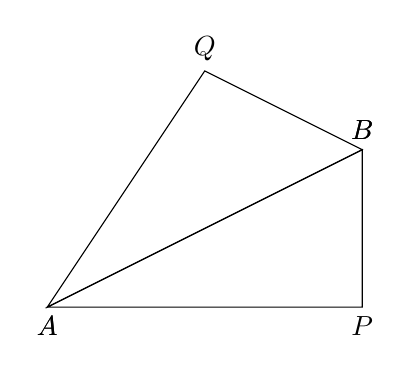
\begin{tikzpicture} 
        \coordinate (P) at (4, 0) {};
        \coordinate (A) at (0, 0) {};
        \coordinate (B) at (4, 2) {};
        \coordinate (Q) at (2, 3) {};
        \draw (Q)node[above]{$Q$}--(A)node[below]{$A$}--(B)node[above]{$B$}--cycle;
        \draw (B)node[above]{$B$}--(A)node[below]{$A$}--(P)node[below]{$P$}--cycle;
\tkzMarkRightAngle[size=.2](B,P,A);
\tkzLabelAngle[dist=.5](P,A,B){};
\tkzMarkRightAngle[size=.2](B,Q,A);
\tkzLabelAngle[dist=.5](Q,A,B){};
\end{tikzpicture}
}
\caption{figure}
\label{eq:solutions/1/25/fig1}
\end{figure}

Given:-
\begin{align}
  \angle{BAP}=\angle{BAQ}=\alpha\label{eq:solutions/1/25/1}\\ 
    \angle{AQB}=\angle{APB}\label{eq:solutions/1/25/2}
\end{align}
In $\triangle ABQ$
\begin{align}
    \angle{ABQ} + \angle{AQB} + \angle{BAQ}=180\degree\label{eq:solutions/1/25/3}
\end{align}
In $\triangle ABP$
\begin{align}
    \angle{ABP} + \angle{APB} + \angle{BAP}=180\degree\label{eq:solutions/1/25/4}
\end{align}
Subtracting \eqref{eq:solutions/1/25/3} and \eqref{eq:solutions/1/25/4} and using \eqref{eq:solutions/1/25/1} and \eqref{eq:solutions/1/25/2} we get,
\begin{align}
\angle{ABQ}=\angle{ABP}
\end{align}
Since,line BP and BQ are perpendicular to AP and AQ respectively..So,their respective dot product will be zero.We get,
\begin{align}
    (\vec{B}-\vec{Q})^T(\vec{A}-\vec{Q})=0\label{eq:solutions/1/25/5}\\
    (\vec{B}-\vec{P})^T(\vec{A}-\vec{P})=0\label{eq:solutions/1/25/6}
\end{align}
We know that,$(\vec{B}-\vec{P})^T(\vec{B}-\vec{P})$ = $\norm{\vec{B}-\vec{P}}^2$\\
 Also let
 \begin{align}
 \norm{\vec{B}-\vec{A}}^2 = k^2\label{eq:solutions/1/25/7}
 \end{align}
\begin{align}
(\vec{B}-\vec{P})^T(\vec{B}-\vec{P})=(\vec{B}-\vec{A}+\vec{A}-\vec{P})^T(\vec{B}-\vec{A}+\vec{A}-\vec{P})
\end{align}
\begin{align}
 \begin{split}
\norm{\vec{B}-\vec{P}}^2=(\vec{B}-\vec{A})^T(\vec{B}-\vec{A})\\
+(\vec{A}-\vec{P})^T(\vec{A}-\vec{P})\\
+(\vec{A}-\vec{P})^T(\vec{B}-\vec{A})\\
+(\vec{B}-\vec{A})^T(\vec{A}-\vec{P})\\
=\norm{\vec{B}-\vec{A}}^2 + \norm{\vec{A}-\vec{P}}^2\\ 
  + 2\norm{\vec{A}-\vec{P}}\norm{\vec{B}-\vec{A}}\cos\alpha\label{eq:solutions/1/25/8}
  \end{split}
\end{align}
\begin{align}
\begin{split}
 (\vec{A}-\vec{P})^T(\vec{B}-\vec{A})=(\vec{B}-\vec{A})^T(\vec{A}-\vec{P})\\
 = \norm{\vec{A}-\vec{P}} \norm{\vec{B}-\vec{A}} \cos\alpha\label{eq:solutions/1/25/18}
\end{split}
\end{align}
Substituting \eqref{eq:solutions/1/25/18}, \eqref{eq:solutions/1/25/7} in \eqref{eq:solutions/1/25/8} we get,
\begin{align}
  \begin{split}
      \norm{\vec{B}-\vec{P}}^2=k^2+\norm{\vec{A}-\vec{P}}^2
      +2k\norm{\vec{A}-\vec{P}}\cos\alpha\label{eq:solutions/1/25/14}
  \end{split}  
\end{align}
Similarly,we get
\begin{align}
    \norm{\vec{B}-\vec{Q}}^2=k^2+\norm{\vec{A}-\vec{Q}}^2
      +2k\norm{\vec{A}-\vec{Q}}\cos\alpha\label{eq:solutions/1/25/15}
\end{align}
\begin{align}
    \cos\alpha = \frac{(\vec{B}-\vec{A})^T(\vec{P}-\vec{A})}{k\norm{\vec{P}-\vec{A}}} = \frac{(\vec{B}-\vec{A})^T(\vec{Q}-\vec{A})}{k\norm{\vec{Q}-\vec{A}}}\label{eq:solutions/1/25/13}\\
    (\vec{B}-\vec{A})^T(\vec{P}-\vec{A})=(\vec{B}-\vec{P}+\vec{P}-\vec{A})^T(\vec{P}-\vec{A})\\
    \implies (\vec{B}-\vec{P})^T(\vec{P}-\vec{A}) + \norm{\vec{P}-\vec{A}}^2\label{eq:solutions/1/25/9}\\
    (\vec{B}-\vec{A})^T(\vec{Q}-\vec{A})=(\vec{B}-\vec{Q}+\vec{Q}-\vec{A})^T(\vec{Q}-\vec{A})\\
     \implies (\vec{B}-\vec{Q})^T(\vec{Q}-\vec{A}) + \norm{\vec{Q}-\vec{A}}^2\label{eq:solutions/1/25/10}
\end{align}
Substituting \eqref{eq:solutions/1/25/5} and \eqref{eq:solutions/1/25/6} in \eqref{eq:solutions/1/25/10} and \eqref{eq:solutions/1/25/9} respectively we get,
\begin{align}
    (\vec{B}-\vec{A})^T(\vec{P}-\vec{A})=\norm{\vec{P}-\vec{A}}^2\label{eq:solutions/1/25/11}\\
    (\vec{B}-\vec{A})^T(\vec{Q}-\vec{A})=\norm{\vec{Q}-\vec{A}}^2\label{eq:solutions/1/25/12}
\end{align}
Substituting \eqref{eq:solutions/1/25/11} and \eqref{eq:solutions/1/25/12} in \eqref{eq:solutions/1/25/13} we get,
\begin{align}
    \norm{\vec{P}-\vec{A}}=\norm{\vec{Q}-\vec{A}}\label{eq:solutions/1/25/16}
\end{align}
Substituting \eqref{eq:solutions/1/25/16} in \eqref{eq:solutions/1/25/14} and \eqref{eq:solutions/1/25/15} we get,
\begin{align}
    \norm{\vec{B}-\vec{P}}=\norm{\vec{B}-\vec{Q}}\label{eq:solutions/1/25/17}
\end{align}
From \eqref{eq:solutions/1/25/17} we can say that $\vec{B}$ is equidistant from the arms of $\angle{A}$,where $\vec{P}$ and $\vec{Q}$ are the points on the arms of $\angle{A}$
Using \eqref{eq:solutions/1/25/1},\eqref{eq:solutions/1/25/2},\eqref{eq:solutions/1/25/17} and by AAS(Angle Angle Side) property of congruency we can say that:-\\
\begin{align}
\triangle APB \cong \triangle AQB
\end{align}
